\documentclass[12pt,a4paper]{article}
% 12pt:     Tamaño de fuente
% a4papper: Tamaño de papel
% article:  Formato artículo, está dividido por secciones y subsecciones. Otros formatos: report, letter, book, etc.

\usepackage[spanish, es-tabla]{babel}
% Configura en español los nombres de figuras, tablas, etc.
\usepackage[utf8]{inputenc}                 % Permite el uso directo de tildes y otros.
\usepackage{amsmath,amssymb}
% Añade símbolos matemáticos para las ecuaciones.
\usepackage{parskip}
% Elimina la sangría
\usepackage{geometry}
% Permite modificar los márgenes de la página a gusto.
\usepackage{multicol}
% Ordena el cuerpo del documento en 2 o más columnas.
\usepackage{graphicx}
% Para poner imágenes.
\usepackage{enumitem}
% Para modificar los tags de los enumerate.
\usepackage{array}
% Para ordenar texto y ecuaciones.
\usepackage{url}
% Permite usar url que redirigen a la página web.
\usepackage{hyperref}
% Permite que se puedan clickear las urls, citas y referencias.

\spanishdecimal{.} % punto decimal
\geometry{margin=2cm} % margenes de la hoja
\renewcommand{\baselinestretch}{1.3} % tamaño de las filas de las tablas

\newcommand{\uveci}{\hat{\imath}} % vector unitario i
\newcommand{\uvecj}{\hat{\jmath}} % vector unitario j
\newcommand{\uveck}{\hat{k}} % vector unitario k

\begin{document}

\begin{center}
{\Large\textbf{INFORME N°2}}

{\LARGE\textbf{Suma vectorial y equilibrio de fuerzas}}

\rule{\textwidth}{0.5pt}

\begin{tabular}{ll}
    \textbf{Estudiantes:} & Juan Ortega \\
                          & Daniel Vallejos \\
                          & Benjamín Moraga \\
                          & Benjamín Montenegro \\[0.2cm]
    \textbf{Profesora:}   & Constanza Rivas \\
    \textbf{Ayudantes:}    & Annelies Fullgraf \\
                                      & Lixin Lai \\[0.2cm]
    \textbf{Fecha de entrega:} & \today
\end{tabular}

\vspace{0.4cm}
\rule{\textwidth}{0.5pt}

\end{center}

\section{Procedimiento experimental}

\subsection{Parte 1 - Mediciones experimentales y suma gráfica de vectores} \label{Procedimiento-Parte-1}

El experimento realizado contaba con una tabla de fuerzas, una balanza, un plumón de pizarra, un resorte enganchado con un pasador rojo, tres cuerdas cortas enganchadas de un extremo al resorte y del otro extremo a unos discos de metal, dos dinamómetros y cuatro masas con gancho idénticas.

\begin{enumerate}[label=\alph*)]

\item Definimos un plano cartesiano de ejes $x$ e $y$, considerando el \textbf{primer cuadrante} en la esquina superior derecha. Tomando en cuenta el \textbf{sentido positivo} de los ángulos como el sentido \textbf{antihorario}. 
\item \textbf{Los ángulos} fueron medidos con la tabla de fuerzas, sirviendo como marco de referencia junto con las cuerdas con las que se ejercía fuerza marcando bajo qué punto de la tabla terminaban las cuerdas; su resolución es $\Delta \theta$ = $5^{\circ}$ sexagesimales. \textbf{Las masas}, se midieron en una balanza de resolución $\Delta m = 0.00001 \,\mathrm{kg}$. 
\item \textbf{Para las fuerzas}, llamamos $F_1$ a la magnitud de la fuerza peso de las masas, por lo tanto $F_1 = m \cdot g$, esto debido a que es la \textbf{fuerza responsable de deformar el resorte} en primer lugar; como la masas con gancho son iguales en forma y magnitud, variar la masa implica multiplicar por la cantidad de masas con gancho que se estén ocupando.
\item Para las tres configuraciones desenganchamos el resorte quitando el pasador rojo para que se deformara por las fuerzas, pero dejándolo aún dentro del resorte para que no sufriera una \textbf{deformación permanente}; mantuvimos fija la fuerza $\vec{F}_1$ al eje $x$ que consideramos positivo \textbf{solo variando la cantidad de masas}; las otras dos fuerzas ($\vec{F}_2$ y $\vec{F}_3$) las medimos con dinamómetros de resolución $\Delta F = 0.01 \,\mathrm{N}$ enganchándolos a los otros anillos,  variando la dirección y el módulo de las fuerzas \textbf{hasta que el pasador volviera a enganchar el resorte}. Ese enganche es el equilibrio de las fuerzas y esas fuerzas \textbf{medidas inmediatamente después} de alcanzar el equilibrio fueron consideradas.
\item Después, usamos dos planos cartesianos en una hoja cuadriculada que coincidieran con el sistema de referencia planteado para los ángulos de las fuerzas por cada configuración, ambos ejes en {\em{Newtons}} ($\mathrm{N}$) con una \textbf{misma escala} $1 \,\mathrm{N}$ para no tener gráficos demasiado grandes y al mismo tiempo que se \textbf{apreciaran bien} los vectores. En el primer gráfico todos los vectores iniciando desde \textbf{el origen}, mientras que en el segundo, solo $\vec{F}_1$ empieza desde el origen, $\vec{F}_2$ comienza desde donde termina $\vec{F}_1$ y $\vec{F}_3$ es la fuerza que finalmente cierra o no por completo el \textbf{polígono. no se consideraron sus errores absolutos}.
\end{enumerate}

\subsection{Parte 2 - Tratamiento analítico y propagación de error} \label{Procedimiento-Parte-2}

Llamamos $F_x$ y $F_y$ a las \textbf{componentes} $x$ e $y$ de las fuerzas respectivamente; para su error absoluto, propagamos el error con \textbf{derivadas parciales} como con cualquier magnitud indirecta, con la diferencia de que $\Delta \theta$ fue convertido a \textbf{radianes} con la relación {\large{$1 \,\mathrm{rad} = \frac{180^{\circ}}{\pi}$}} debido a que las funciones trigonométricas están definidas en radianes. 

Para las componentes $x$:
\begin{align*}
F_x &= F \cos\theta \\
\Delta F_x &= \sqrt{\left(\frac{\partial F_x}{\partial F}\Delta F\right)^2 + \left(\frac{\partial F_x}{\partial \theta}\Delta \theta_{\text{rad}}\right)^2} = \sqrt{\left(\cos\theta \, \Delta F\right)^2 + \left(-F\sin\theta \, \left(\Delta \theta \frac{\pi}{180^\circ}\right)\right)^2}
\end{align*}

Para las componentes $y$:
\begin{align*}
    F_y &= F \sin\theta \\
    \Delta F_y &= \sqrt{\left(\frac{\partial F_y}{\partial F}\Delta F\right)^2 + \left(\frac{\partial F_y}{\partial \theta}\Delta \theta_{\text{rad}}\right)^2} = \sqrt{\left(\sin\theta \, \Delta F\right)^2 + \left(F\cos\theta \, \left(\Delta \theta \frac{\pi}{180^\circ}\right)\right)^2}
\end{align*}

El vector resultante ($\vec{R}$) resulta de la \textbf{suma vectorial} de las fuerzas, las separamos en sus componentes $x$ e $y$ para definir $R_x$ y $R_y$ las \textbf{componentes} de $\vec{R}$, quedando:

\begin{align*}
R_x &= F_{1x} + F_{2x} + F_{3x}, \qquad \Delta R_x = \sqrt{\Delta F_{1x}^2 + \Delta F_{2x}^2 + \Delta F_{3x}^2} \\
R_y &= F_{1y} + F_{2y} + F_{3y}, \qquad \Delta R_y = \sqrt{\Delta F_{1y}^2 + \Delta F_{2y}^2 + \Delta F_{3y}^2}
\end{align*}

Para el caso de $F_1$, su error no está asociado a ningún dinamómetro sino a una propagación de errores de modo que:

\begin{align*}
    F_1 &= m g \\
    \Delta F_1 &= \sqrt{\left(\frac{\partial F_1}{\partial m}\Delta m\right)^2 + \left(\frac{\partial F_1}{\partial g}\Delta g\right)^2} = \sqrt{\left(g \, \Delta m\right)^2 + \left(m \, \Delta g\right)^2}
\end{align*}
\subsection{Parte 3 - Comparación con la predicción teórica y análisis gráfico} \label{Procedimiento-Parte-3}

Los gráficos de los vectores resultantes $R_x$ y $R_y$ se hicieron en Python teniendo en cuenta cosas como:

\begin{enumerate}[label=\alph*)]
\item El eje $x$ se definió como una \textbf{lista} de los elementos $R_x$ y $R_y$, mostrando los errores de cada componente por separado sin problemas \textbf{(variable independiente)}. Los puntos del eje $y$ representan los valores que pueden tomar las componentes resultantes en N \textbf{(variable dependiente)}; la escala en $y$ no es la misma en cada configuración puesto que los vectores resultantes y sus errores variaban, no obstante, se mantuvo la misma separación por puntos y todos los gráficos incluyen el punto $y = 0 \,\mathrm{N}$.
\item Con Python, nos apoyamos de \textbf{plt.errorbar()} y definimos el valor medido y el error \textbf{(y, yerr respectivamente)} como listas de dos elementos, con el objeto de que coincidan para $R_x$ y $R_y$.
\item En la misma línea de comandos, ingresamos una \textbf{recta constante} definida desde $R_x$ hasta $R_y$ de modo que sus imágenes tomaran valores $y = 0 \,\mathrm{N}$ para cada punto. Dicha recta visualiza si el vector resultante \textbf{pasa por el $0 \mathrm{N}$ o no}, lo cual significa el equilibrio de fuerzas.
\item Si $R_x$ y $R_y$ pasan por la recta, los resultados son \textbf{compatibles} con el equilibrio, esto a causa de que sus valores se encuentran en sus rangos de error ($x = \bar{x} \pm \Delta x$), por lo tanto se puede considerar que el el vector resultante $\vec{R}$ es un vector \textbf{nulo}.
\end{enumerate}

\newpage

% Fin parte 1 _______________________________________________________________________________________________________________________________________________________________

\section{Configuración de Equilibrio 1}

Describan brevemente la primera configuración de equilibrio, considerando la cantidad de masas suspendidas, la disposición de los dinamómetros y los ángulos seleccionados.

\begin{table}[h!]
\centering
\begin{tabular}{|c|c|c|}
\hline
\textbf{Fuerza} & \textbf{Módulo ($F \pm \delta F$)} & \textbf{Ángulo ($\theta \pm \delta \theta$)} \\ \hline
$F_1$ & & \\ \hline
$F_2$ & & \\ \hline
$F_3$ & & \\ \hline
\end{tabular}
\caption{Medición directa e indirecta de módulos y ángulos para la Configuración 1.}
\label{tab:config1-mediciones}
\end{table}

Los datos recolectados de esta configuración fueron registrados en la Tabla \ref{tab:config1-mediciones}. La representación gráfica de los vectores de esta configuración se puede ver en la Fig. \ref{fig:config1-vectores}.

\begin{figure}[h!]
    \centering
    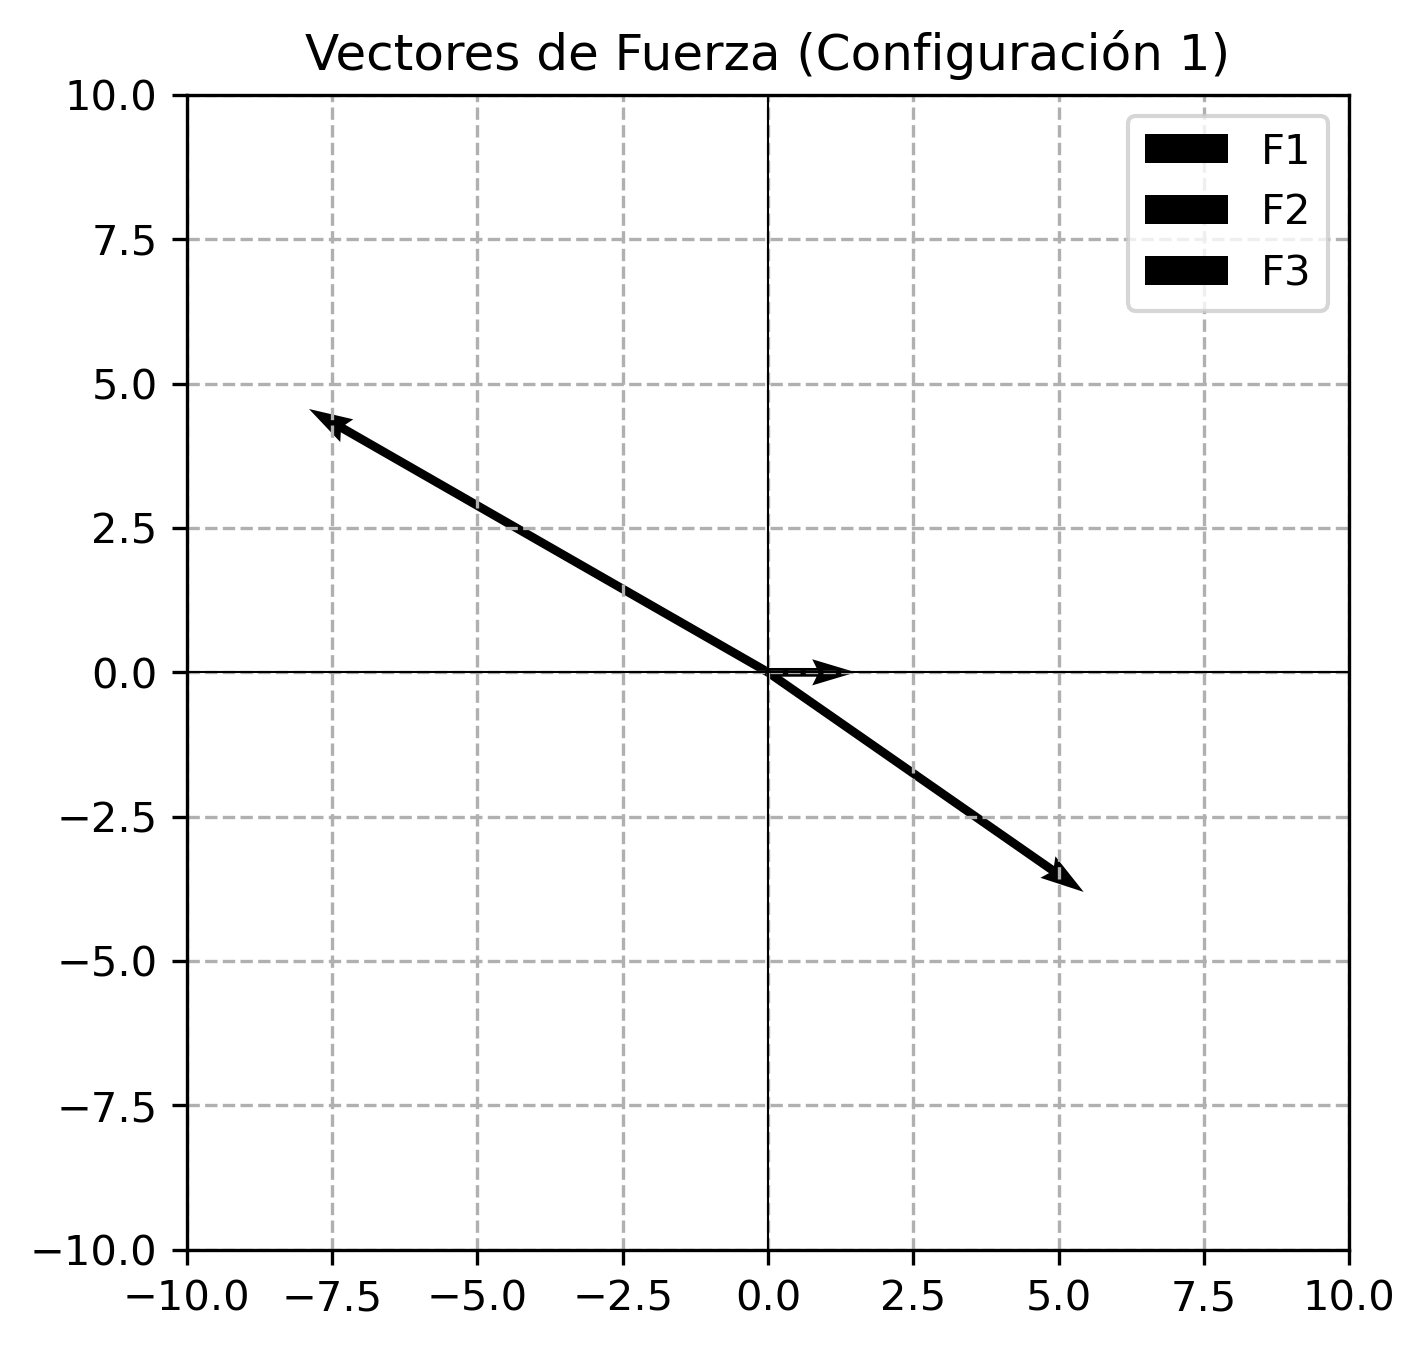
\includegraphics[width=0.4\textwidth]{config1-vectores.png}
    \caption{Representación en el sistema de referencia de los vectores $\vec{F}_1$, $\vec{F}_2$ y $\vec{F}_3$ (Configuración 1).}
    \label{fig:config1-vectores}
\end{figure}

El módulo de $\vec{F}_1$ corresponde al peso de la masa, calculado como $F_1 = mg$. Para obtener $\delta F_1$, se realizó propagación de error.
\begin{equation*}
F_1 = mg = \dots
\end{equation*}
\begin{equation*}
\delta F_1 = \sqrt{\left(\frac{\partial F}{\partial m} \Delta m \right)^2 + \left(\frac{\partial F}{\partial g} \Delta g \right)^2} = \dots
\end{equation*}

\subsection{Suma gráfica}

La suma gráfica de los vectores se puede ver en la Fig. \ref{fig:config1-poligono}.

\begin{figure}[h!]
    \centering
    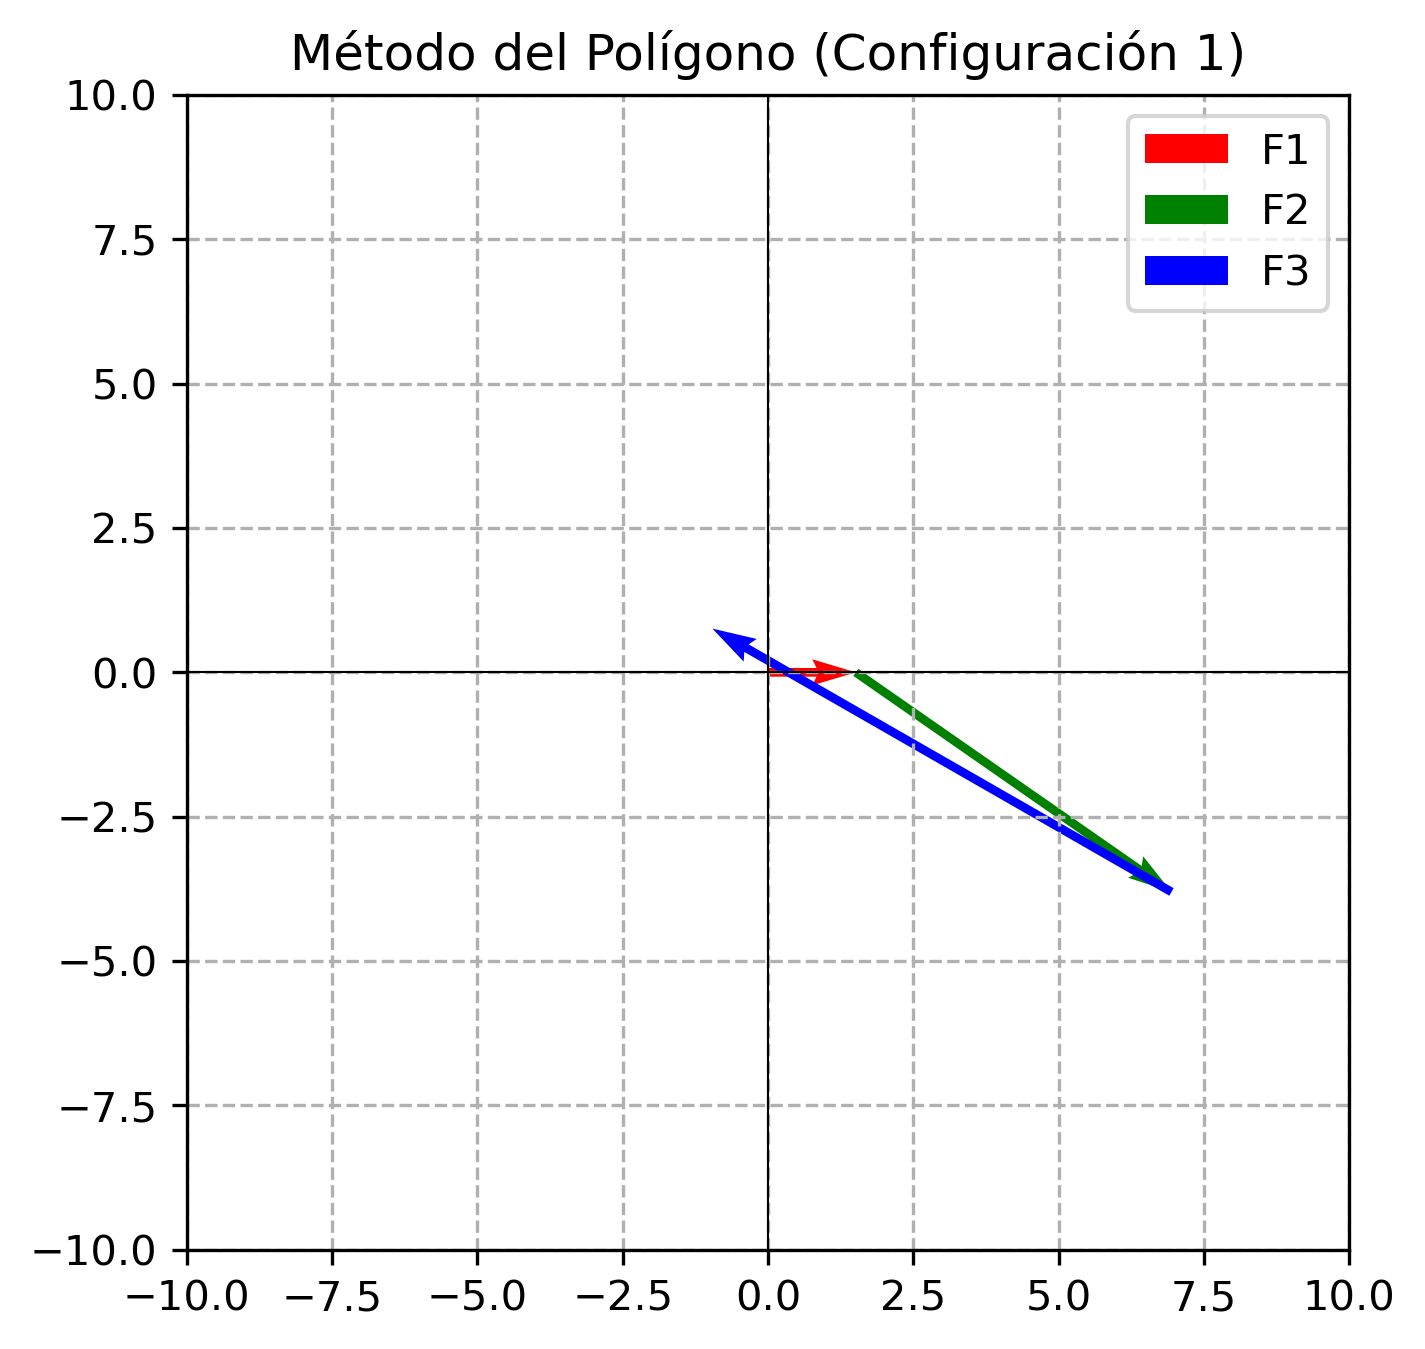
\includegraphics[width=0.4\textwidth]{config1-poligono.png}
    \caption{Suma gráfica mediante el método del polígono para la Configuración 1.}
    \label{fig:config1-poligono}
\end{figure}

Comenten cualitativamente si el polígono se cierra correctamente o si existe alguna discrepancia gráfica visible.

\subsection{Suma analítica}

Los vectores de la Configuración 1 separados en sus componentes están registrados en la Tabla \ref{tab:config1-componentes}.

\begin{table}[h!]
\centering
\begin{tabular}{|c|c|c|}
\hline
\textbf{Fuerza} & $F_x \pm \Delta F_x\,\mathrm{(N)}$ & $F_y \pm \Delta F_y\,\mathrm{(N)}$ \\ \hline
$F_1$ & & \\ \hline
$F_2$ & & \\ \hline
$F_3$ & & \\ \hline
\end{tabular}
\caption{Componentes cartesianas e incertidumbres absolutas para la Configuración 1.}
\label{tab:config1-componentes}
\end{table}

Sumando estas componentes, el vector resultante es:

\begin{equation*}
\vec{R}_{\mathrm{exp, 1}} = (R_x \pm \Delta R_x)\,\uveci + (R_y \pm \Delta R_y)\,\uvecj = (\dots \pm \dots)\,\uveci + (\dots \pm \dots)\,\uvecj\,\mathrm{N}
\end{equation*}

\subsection{Comparación de los resultados}

La Fig. \ref{fig:grafico-error-1} muestra la comparación gráfica entre la predicción teórica y el resultado experimental.

\begin{figure}[h!]
    \centering
    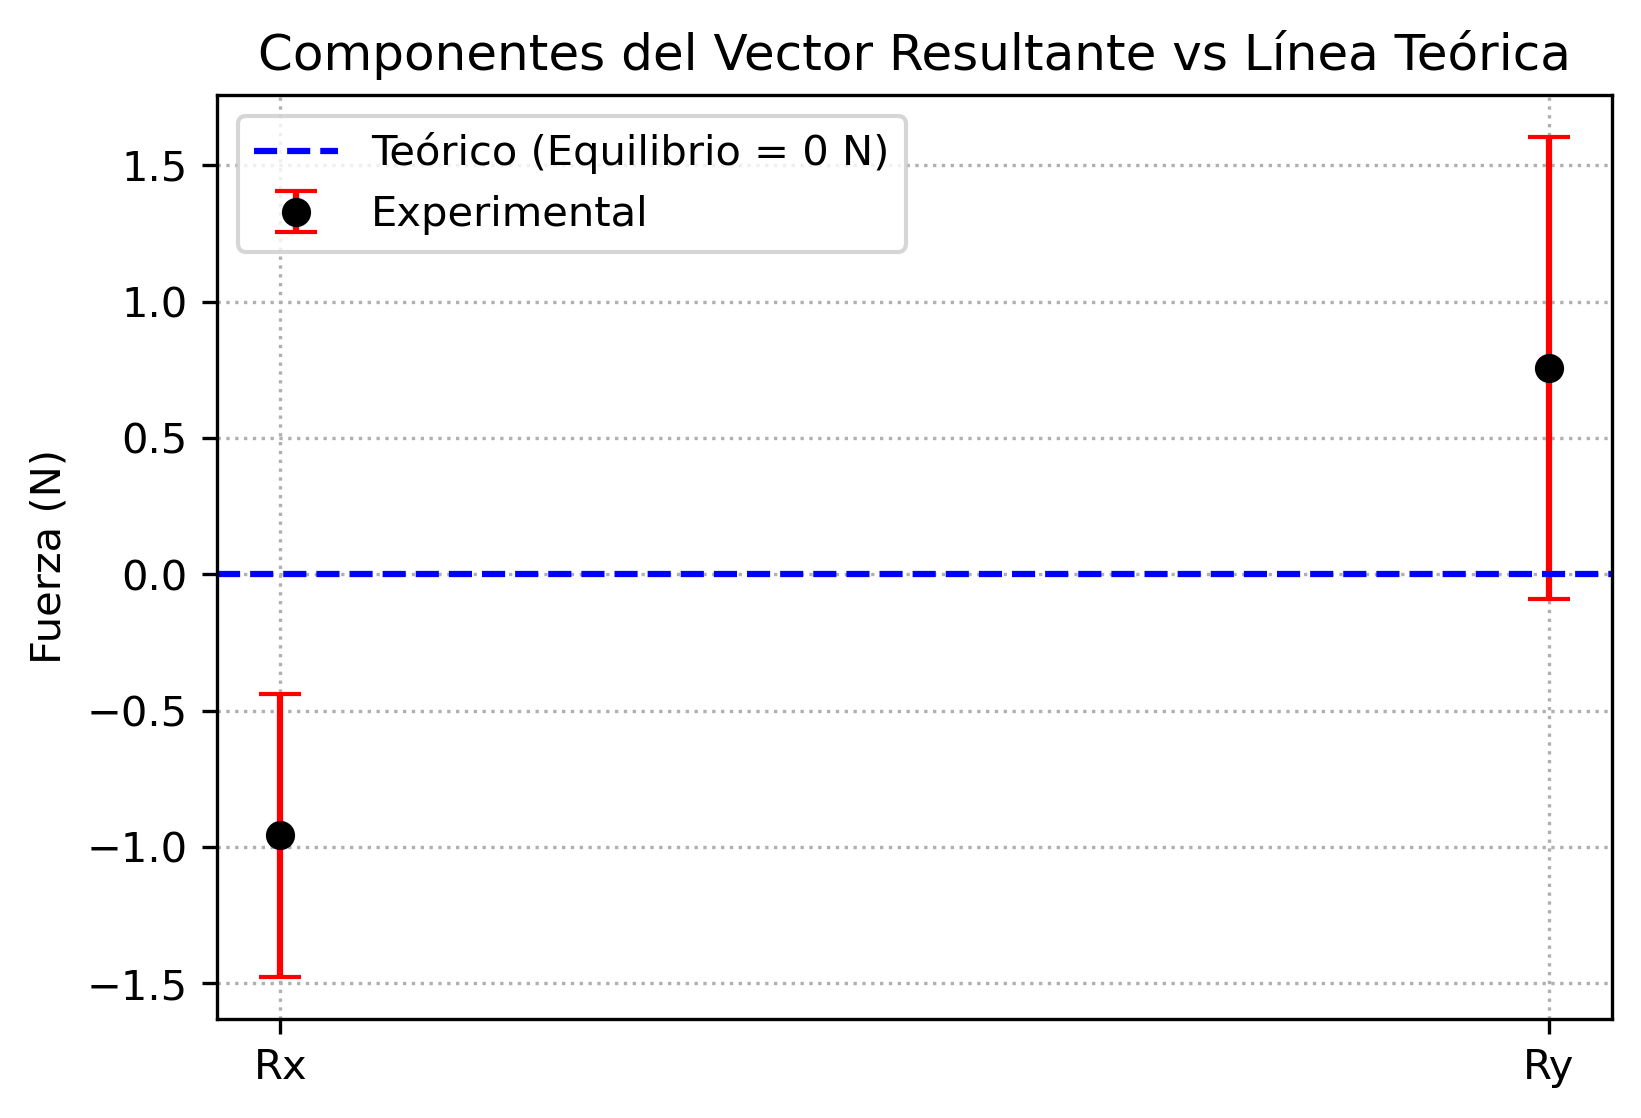
\includegraphics[width=0.4\textwidth]{grafico-error-config1.png}
    \caption{Gráficos de las componentes de la fuerza resultante $R_x$ y $R_y$ con barras de error en relación a la referencia teórica $y=0\,\mathrm{N}$ para la Configuración 1.}
    \label{fig:grafico-error-1}
\end{figure}

Describan y analicen el gráfico obtenido. Indiquen si las barras de error de las componentes $R_x$ y $R_y$ cruzan la línea de referencia $y = 0\,\mathrm{N}$ y qué concluyen a partir de dicho cruce sobre la compatibilidad experimental con la condición de equilibrio traslacional.

\newpage

\section{Configuración de Equilibrio 2}

Describan la segunda configuración de equilibrio utilizada, considerando la cantidad de masas suspendidas, la disposición de los dinamómetros y los ángulos seleccionados.

\begin{table}[h!]
\centering
\begin{tabular}{|c|c|c|}
\hline
\textbf{Fuerza} & \textbf{Módulo ($F \pm \delta F$)} & \textbf{Ángulo ($\theta \pm \delta \theta$)} \\ \hline
$F_1$ & & \\ \hline
$F_2$ & & \\ \hline
$F_3$ & & \\ \hline
\end{tabular}
\caption{Medición directa e indirecta de módulos y ángulos para la Configuración 2.}
\label{tab:config2-mediciones}
\end{table}

Los datos recolectados de esta configuración fueron registrados en la Tabla \ref{tab:config2-mediciones}. El módulo de $\vec{F}_1$ corresponde al peso de la masa, calculado como $F_1 = mg$. Para obtener $\delta F_1$, se realizó propagación de error.

\begin{equation*}
F_1 = mg = \dots
\end{equation*}
\begin{equation*}
\delta F_1 = \sqrt{\left(\frac{\partial F}{\partial m} \Delta m \right)^2 + \left(\frac{\partial F}{\partial g} \Delta g \right)^2} = \dots
\end{equation*}

La representación gráfica de los vectores de esta configuración se puede ver en la Fig. \ref{fig:config2-vectores}.

\begin{figure}[h!]
    \centering
    \includegraphics[width=0.4\textwidth]{config2-vectores.png}
    \caption{Representación en el sistema de referencia de los vectores $\vec{F}_1$, $\vec{F}_2$ y $\vec{F}_3$ (Configuración 2).}
    \label{fig:config2-vectores}
\end{figure}

\subsection{Suma gráfica de los vectores de la Configuración 2}

La suma gráfica de los vectores se puede ver en la Fig. \ref{fig:config2-poligono}.

\begin{figure}[h!]
    \centering
    \includegraphics[width=0.4\textwidth]{config2-poligono.png}
    \caption{Suma gráfica mediante el método del polígono para la Configuración 2.}
    \label{fig:config2-poligono}
\end{figure}

Comenten cualitativamente si el polígono se cierra correctamente o si existe alguna discrepancia gráfica visible.

\subsection{Suma analítica}

Los vectores de la Configuración 2 separados en sus componentes están registrados en la Tabla \ref{tab:config2-componentes}.

\begin{table}[h!]
\centering
\begin{tabular}{|c|c|c|}
\hline
\textbf{Fuerza} & $F_x \pm \Delta F_x\,\mathrm{(N)}$ & $F_y \pm \Delta F_y\,\mathrm{(N)}$ \\ \hline
$F_1$ & & \\ \hline
$F_2$ & & \\ \hline
$F_3$ & & \\ \hline
\end{tabular}
\caption{Componentes cartesianas e incertidumbres absolutas para la Configuración 2.}
\label{tab:config2-componentes}
\end{table}

Sumando estas componentes, el vector resultante es:

\begin{equation*}
\vec{R}_{\mathrm{exp, 2}} = (R_x \pm \Delta R_x)\,\uveci + (R_y \pm \Delta R_y)\,\uvecj = (\dots \pm \dots)\,\uveci + (\dots \pm \dots)\,\uvecj\,\mathrm{N}
\end{equation*}

\subsection{Comparación de los resultados}

La Fig. \ref{fig:grafico-error-2} muestra la comparación gráfica entre la predicción teórica y el resultado experimental.

\begin{figure}[h!]
    \centering
    \includegraphics[width=0.4\textwidth]{grafico-error-config2.png}
    \caption{Gráficos de las componentes de la fuerza resultante $R_x$ y $R_y$ con barras de error en relación a la referencia teórica $y=0\,\mathrm{N}$ para la Configuración 2.}
    \label{fig:grafico-error-2}
\end{figure}

Describan y analicen el gráfico obtenido. Indiquen si las barras de error de las componentes $R_x$ y $R_y$ cruzan la línea de referencia $y = 0\,\mathrm{N}$ y qué concluyen a partir de dicho cruce sobre la compatibilidad experimental con la condición de equilibrio traslacional.

\newpage
\section{Configuración de Equilibrio 3}

Describan la tercera configuración de equilibrio utilizada, considerando la cantidad de masas suspendidas, la disposición de los dinamómetros y los ángulos seleccionados.

\begin{table}[h!]
\centering
\begin{tabular}{|c|c|c|}
\hline
\textbf{Fuerza} & \textbf{Módulo ($F \pm \delta F$)} & \textbf{Ángulo ($\theta \pm \delta \theta$)} \\ \hline
$F_1$ & & \\ \hline
$F_2$ & & \\ \hline
$F_3$ & & \\ \hline
\end{tabular}
\caption{Medición directa e indirecta de módulos y ángulos para la Configuración 3.}
\label{tab:config3-mediciones}
\end{table}

Los datos recolectados de esta configuración fueron registrados en la Tabla \ref{tab:config3-mediciones}. El módulo de $\vec{F}_1$ corresponde al peso de la masa, calculado como $F_1 = mg$. Para obtener $\delta F_1$, se realizó propagación de error.
\begin{equation*}
F_1 = mg = \dots
\end{equation*}
\begin{equation*}
\delta F_1 = \sqrt{\left(\frac{\partial F}{\partial m} \Delta m \right)^2 + \left(\frac{\partial F}{\partial g} \Delta g \right)^2} = \dots
\end{equation*}

La representación gráfica de los vectores de esta configuración se puede ver en la Fig. \ref{fig:config3-vectores}.

\begin{figure}[h!]
    \centering
    \includegraphics[width=0.4\textwidth]{config3-vectores.png}
    \caption{Representación en el sistema de referencia de los vectores $\vec{F}_1$, $\vec{F}_2$ y $\vec{F}_3$ (Configuración 3).}
    \label{fig:config3-vectores}
\end{figure}

\subsection{Suma gráfica de los vectores de la Configuración 3}

La suma gráfica de los vectores se puede ver en la Fig. \ref{fig:config3-poligono}.

\begin{figure}[h!]
    \centering
    \includegraphics[width=0.4\textwidth]{config3-poligono.png}
    \caption{Suma gráfica mediante el método del polígono para la Configuración 3.}
    \label{fig:config3-poligono}
\end{figure}

Comenten cualitativamente si el polígono se cierra correctamente o si existe alguna discrepancia gráfica visible.

\subsection{Suma analítica de los vectores de la Configuración 3}

Los vectores de la Configuración 3 separados en sus componentes están registrados en la Tabla \ref{tab:config3-componentes}.

\begin{table}[h!]
\centering
\begin{tabular}{|c|c|c|}
\hline
\textbf{Fuerza} & $F_x \pm \Delta F_x\,\mathrm{(N)}$ & $F_y \pm \Delta F_y\,\mathrm{(N)}$ \\ \hline
$F_1$ & & \\ \hline
$F_2$ & & \\ \hline
$F_3$ & & \\ \hline
\end{tabular}
\caption{Componentes cartesianas e incertidumbres absolutas para la Configuración 3.}
\label{tab:config3-componentes}
\end{table}

Sumando estas componentes, el vector resultante es:

\begin{equation*}
\vec{R}_{\mathrm{exp, 3}} = (R_x \pm \Delta R_x)\,\uveci + (R_y \pm \Delta R_y)\,\uvecj = (\dots \pm \dots)\,\uveci + (\dots \pm \dots)\,\uvecj\,\mathrm{N}
\end{equation*}

\subsection{Comparación de los resultados}

La Fig. \ref{fig:grafico-error-3} muestra la comparación gráfica entre la predicción teórica y el resultado experimental.

\begin{figure}[h!]
    \centering
    \includegraphics[width=0.4\textwidth]{grafico-error-config3.png}
    \caption{Gráficos de las componentes de la fuerza resultante $R_x$ y $R_y$ con barras de error en relación a la referencia teórica $y=0\,\mathrm{N}$ para la Configuración 3.}
    \label{fig:grafico-error-3}
\end{figure}

Describan y analicen el gráfico obtenido. Indiquen si las barras de error de las componentes $R_x$ y $R_y$ cruzan la línea de referencia $y = 0\,\mathrm{N}$ y qué concluyen a partir de dicho cruce sobre la compatibilidad experimental con la condición de equilibrio traslacional.

\newpage
\section{Análisis y conclusiones}

En la presente experiencia de laboratorio se estudió la suma vectorial y las condiciones de equilibrio traslacional de fuerzas coplanares concurrentes. Para ello, en la primera parte se implementaron tres configuraciones experimentales distintas utilizando una mesa de fuerzas, masas suspendidas, dinamómetros y poleas, registrando los módulos y ángulos de tres vectores de fuerza ($\vec{F}_1$, $\vec{F}_2$ y $\vec{F}_3$) por cada configuración (Secciones 2, 3 y 4; Tablas 1, 2 y 3). En la segunda parte, se realizó el tratamiento analítico calculando el peso de la masa mediante la relación $F_1 = mg$ con su respectiva propagación de error, determinando las componentes cartesianas ($F_x, F_y$) y sus incertidumbres absolutas ($\Delta F_x, \Delta F_y$), para finalmente hallar el vector resultante experimental $\vec{R}_{\text{exp}}$ y los errores asociados $\Delta R_x$ y $\Delta R_y$. Finalmente, en la tercera parte, se construyeron representaciones gráficas mediante el método del polígono y gráficos de puntos con barras de error en Python para las componentes $R_x$ y $R_y$, evaluando su compatibilidad con la predicción teórica de equilibrio ($y = 0\,\mathrm{N}$).   El análisis físico de los resultados permite comprender que la expresión $\sum \vec{F}_i = \vec{F}_1 + \vec{F}_2 + \vec{F}_3 = \vec{0}$ representa la primera condición de equilibrio traslacional, la cual postula que la fuerza neta o resultante que actúa sobre un punto material debe ser nula para que este permanezca en reposo o con velocidad constante. Al comparar los métodos gráficos con los analíticos, se observa que aunque el método del polígono (Figuras 2, 5 y 8) permite visualizar de manera rápida e intuitiva si el sistema se encuentra en equilibrio mediante el cierre del polígono, el tratamiento analítico combinado con la propagación de errores proporciona un rigor cuantitativo muy superior. Esto último se debe a que la suma gráfica está limitada por la precisión visual y la escala del trazado, mientras que el cálculo analítico y los gráficos de barras de error consideran de forma estricta las incertidumbres instrumentales y de medición. Al examinar las componentes del vector resultante en las tres configuraciones, se advierte que los valores obtenidos no son exactamente cero ($R_x \neq 0$ y $R_y \neq 0$); sin embargo, esto no contradice la teoría, ya que en un entorno experimental las mediciones arrastran errores inherentes debido a la resolución de los instrumentos (como la tabla de fuerza y los dinamómetros) y a factores como la fricción estática en las poleas. No obstante, al graficar los resultados con sus respectivas barras de error e incorporarlas en relación con la línea de referencia teórica en $y = 0\,\mathrm{N}$, se constata que las barras de error cruzan dicha línea de referencia en las configuraciones evaluadas. Esta intersección aporta información concluyente, ya que indica que las discrepancias observadas son estadísticamente compatibles con cero dentro del intervalo de confianza considerado, validando experimentalmente la condición de equilibrio traslacional del sistema. Al contrastar las tres configuraciones experimentales, se aprecia que comparten la misma estructura metodológica de equilibrio con tres fuerzas concurrentes, pero varían en la magnitud de las masas y en las orientaciones angulares seleccionadas, demostrando que la condición de equilibrio se satisface independientemente de la distribución geométrica de los vectores siempre que sus componentes vectoriales se anulen mutuamente. Pese a los resultados favorables, se identificaron fuentes de error experimental relevantes que afectaron la precisión de la práctica, tales como el paralaje al medir los ángulos con la tabla de fuerzas, la fricción en los ejes de las poleas que impide una libertad de movimiento perfecta y pequeñas desviaciones en la alineación del resorte y las cuerdas respecto al plano horizontal de la tabla.   Como grupo, a partir del trabajo realizado se concluye que la verificación experimental de leyes físicas fundamentales requiere obligatoriamente de un análisis riguroso de errores y no solo de la obtención de valores nominales ideales, ya que la concordancia entre la teoría y la práctica se define en términos de compatibilidad estadística y no de una igualdad absoluta. Asimismo, se destaca la importancia de las herramientas de representación gráfica, como los diagramas vectoriales y los gráficos de error con Python, para interpretar de manera clara y visual si los resultados se ajustan a los modelos teóricos esperados. Finalmente, se reconoce que el control adecuado de las fuentes de incertidumbre experimental y la correcta elección de las escalas de medida son determinantes para minimizar las desviaciones y optimizar la precisión en el estudio de sistemas mecánicos en equilibrio. 

\textbf{\underline{Extensión máxima del informe:} indefinida}.

\begin{thebibliography}{99}

\bibitem{libro} Nombre del autor. \textit{Título del libro}. Año.

\bibitem{apunte} Nombre del profesor. \textit{Nombre del curso}. Semestre y año en el que fue entregado el apunte.

\bibitem{web} TikTok de @usuario. Disponible en: \url{https://www.tiktok.com/}.

\end{thebibliography}

\end{document}
